\documentclass[12pt]{article}
\usepackage[utf8]{inputenc}
\usepackage{graphicx}
\usepackage{amsmath}
\usepackage{geometry}
\usepackage{float}
\geometry{margin=2.5cm}

\title{BLG 527E – Deep Learning \\ Homework 2 Report}
\author{Ahmed Senih Yıldırım  504241568}
\date{\today}

\begin{document}
\maketitle

\section*{Introduction}

This report summarizes the experiments and results from Homework 2 of the BLG 527E Deep Learning course. Two deep learning tasks were implemented using the Fashion-MNIST dataset: (1) Autoencoder for image reconstruction and generation, and (2) Feedforward Neural Network (FFNN) for image classification.

\section*{Question 1: Autoencoder – Reconstruction and Generation}

\subsection*{1.1 Architecture and Hyperparameters}

A deep fully connected autoencoder was implemented. The encoder compresses a flattened 28x28 grayscale image into a 64-dimensional latent vector. The decoder reconstructs the original image from this representation.

\begin{itemize}
    \item \textbf{Encoder:}
    \begin{itemize}
        \item Flatten → Linear(784, 512) → ReLU
        \item Linear(512, 256) → ReLU
        \item Linear(256, 64)
    \end{itemize}
    \item \textbf{Decoder:}
    \begin{itemize}
        \item Linear(64, 256) → ReLU
        \item Linear(256, 512) → ReLU
        \item Linear(512, 784) → Sigmoid → Unflatten to (1, 28, 28)
    \end{itemize}
\end{itemize}




\textbf{Training parameters:}

\begin{itemize}
    \item Epochs: 50
    \item Batch Size: 128
    \item Optimizer: Adam
    \item Learning Rate: 0.001
    \item Loss Function: Mean Squared Error (MSE)
    \item Scheduler: StepLR with gamma = 0.5 every 10 epochs
    \item Device: CUDA (if available)
\end{itemize}

\subsection*{1.2 Design Motivation}

The architecture is fully connected for simplicity and because Fashion-MNIST images are small and low-dimensional. ReLU activations allow non-linear encoding, and Sigmoid matches the pixel range [0, 1]. We used a Denoising Autoencoder setup by adding Gaussian noise to the input, encouraging the model to learn more robust features.

\subsection*{1.3 Training and Final Loss}

The model was trained on the Fashion-MNIST training set for 50 epochs. The training loss decreased consistently, showing smooth convergence.

\begin{center}
\textbf{Final Test Reconstruction Loss: 0.0099}
\end{center}

\begin{figure}[H]
    \centering
    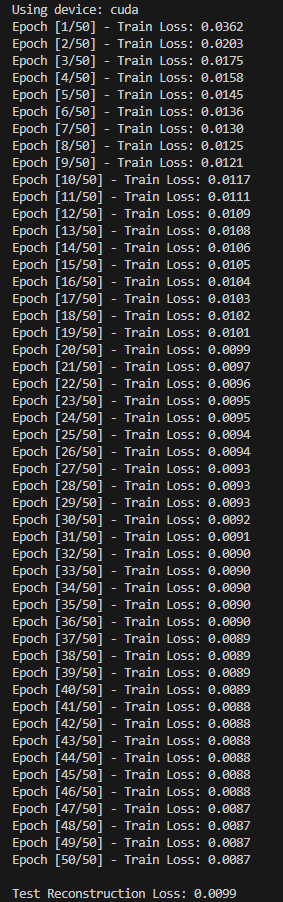
\includegraphics[width=0.35\linewidth]{question1_test_scores.png}
    \caption{Training Output Log for Autoencoder (Epoch-wise Loss)}
\end{figure}

\subsection*{1.4 Reconstruction Results}

Below are examples of original and reconstructed test images. Although fine-grained textures are sometimes blurred, global structure is preserved.

\begin{figure}[H]
    \centering
    \includegraphics[width=1.0\linewidth]{reconstruction_result.png}
    \caption{Original (top) vs. Reconstructed (bottom) Images}
\end{figure}

\subsection*{1.5 Generated Samples from Latent Space}

To evaluate generative capability, we sampled random vectors from a normal distribution and decoded them. Some resemble clothing items, while others are less realistic, which is expected from vanilla AEs.

\begin{figure}[H]
    \centering
    \includegraphics[width=0.9\linewidth]{question1_samples.png}
    \caption{Generated Samples from Random Latent Vectors}
\end{figure}

\subsection*{Note on Dataset Loading}

Instead of using the standard `torchvision.datasets.FashionMNIST` class, a custom dataset loader named \texttt{FashionMNISTFromFile} was used. This class reads the raw binary \texttt{.gz} files using a utility script (\texttt{mnist\_reader.py}) and loads the data into PyTorch tensors manually. Pixel values are normalized to the range [0, 1], and images are reshaped into \texttt{(1, 28, 28)} to match expected input shapes.

This approach follows the dataset usage specified in the original repository and satisfies the assignment requirement to use the raw Fashion-MNIST files directly.


\section*{Question 2: FFNN Classification}

\subsection*{2.1 Architecture and Hyperparameters}

A feedforward neural network with 3 hidden layers was used for classification.

\begin{itemize}
    \item Input: Flatten(28x28) → 784
    \item Linear(784, 512) → BatchNorm → ReLU → Dropout(0.2)
    \item Linear(512, 256) → BatchNorm → ReLU → Dropout(0.2)
    \item Linear(256, 128) → ReLU
    \item Output: Linear(128, 10)
\end{itemize}

\textbf{Training configuration:}

\begin{itemize}
    \item Epochs: 50
    \item Batch Size: 128
    \item Optimizer: Adam
    \item Loss Function: CrossEntropyLoss
    \item Learning Rate: 0.001
\end{itemize}

\subsection*{2.2 Design Motivation}

Batch Normalization speeds up training by stabilizing layer outputs, while Dropout prevents overfitting. ReLU activations improve gradient flow. Despite the simple architecture, the model handles Fashion-MNIST effectively without convolutions.

\subsection*{2.3 Training Performance}

The model converged smoothly, achieving high accuracy without overfitting.

\begin{center}
\textbf{Final Test Accuracy: 90.10\%}
\end{center}

\begin{figure}[H]
    \centering
    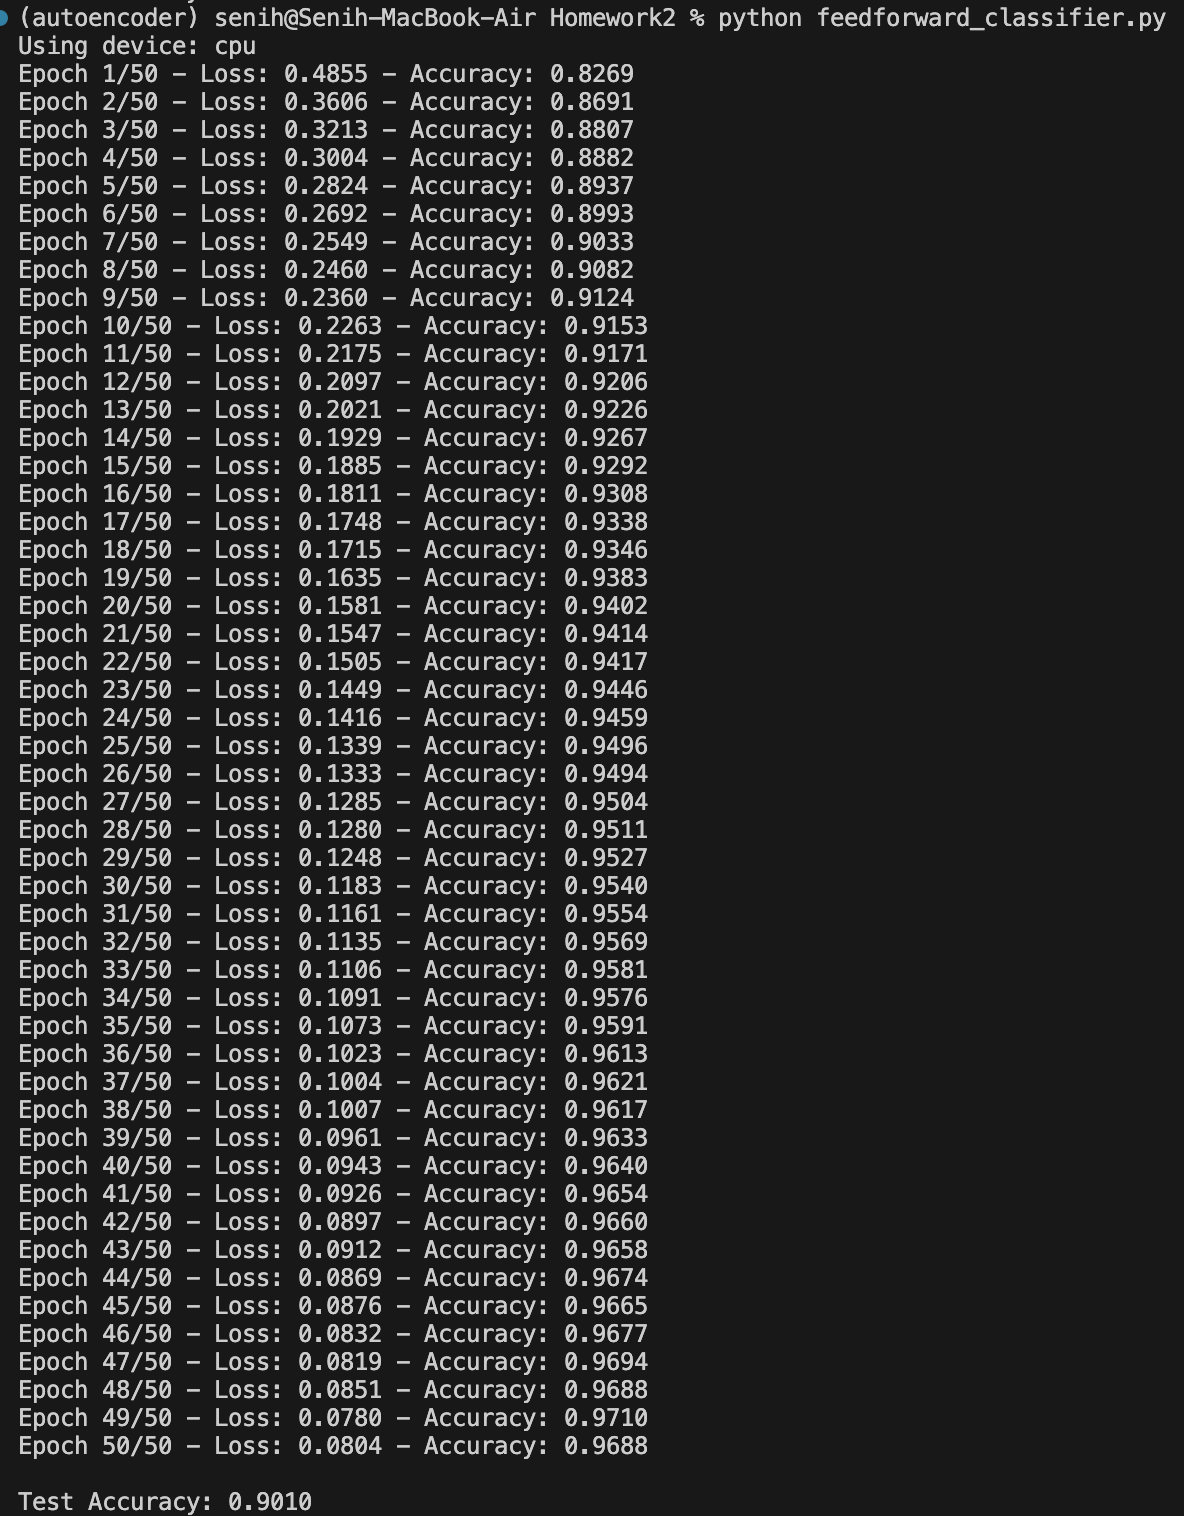
\includegraphics[width=0.9\linewidth]{question2_test_scores.png}
    \caption{Training Loss and Accuracy per Epoch}
\end{figure}

\subsection*{2.4 Confusion Matrix}

The matrix shows high overall performance. Most errors happen between visually similar classes such as Shirt vs. T-shirt or Coat vs. Pullover.

\begin{figure}[H]
    \centering
    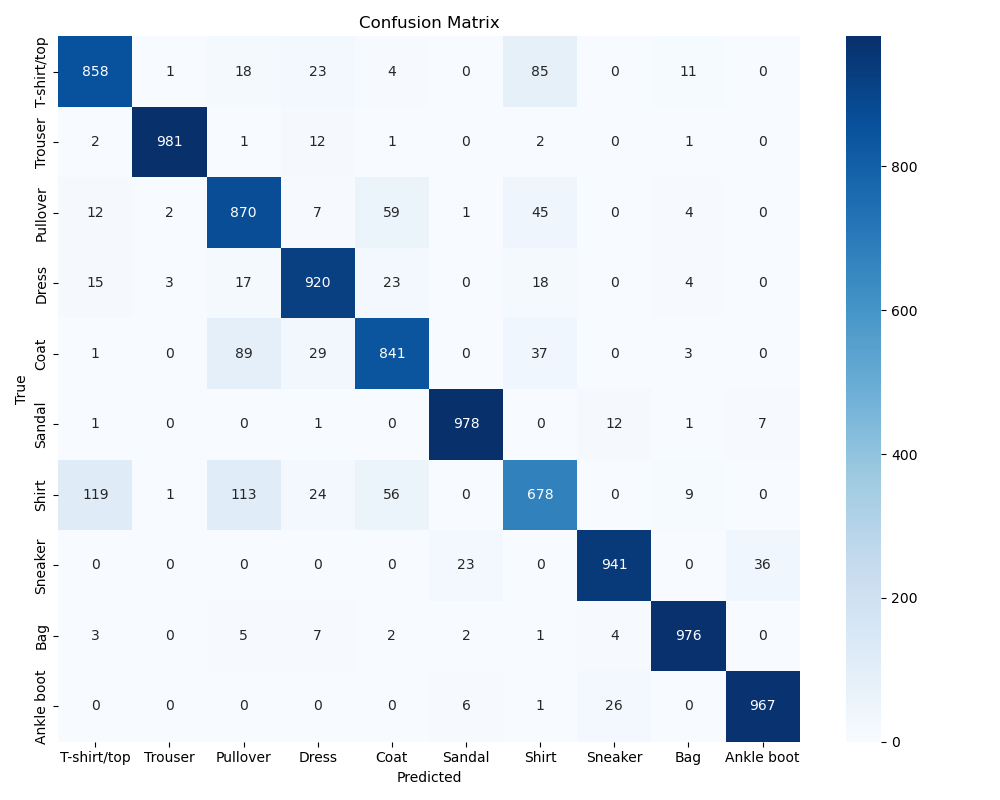
\includegraphics[width=0.9\linewidth]{Figure_1.png}
    \caption{Confusion Matrix: Predicted vs Ground Truth}
\end{figure}

\subsection*{2.5 Misclassified Samples}

Sample misclassifications are visualized below. Despite some errors, most predictions are reasonable and often close to the true class.

\begin{figure}[H]
    \centering
    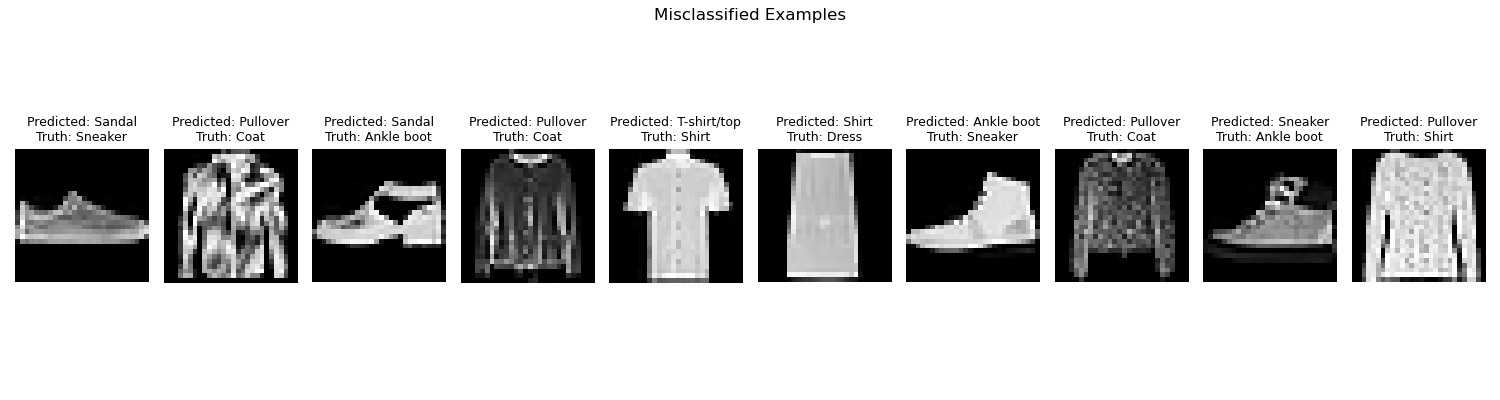
\includegraphics[width=0.9\linewidth]{Figure_2.png}
    \caption{Examples of Misclassified Test Images}
\end{figure}

\section*{Conclusion}

In this assignment, two deep learning models were developed and evaluated on the Zalando Fashion-MNIST dataset. The first task focused on unsupervised learning using a deep autoencoder architecture for image compression, reconstruction, and sample generation. Training with added Gaussian noise improved the robustness of the model. The final reconstruction loss was low, indicating that the model successfully learned to represent image structures, although generated samples lacked sharpness due to the limitations of vanilla autoencoders.

The second task tackled a supervised image classification problem using a feedforward neural network. The architecture was enhanced with Batch Normalization and Dropout layers to prevent overfitting. The model achieved a final test accuracy of around 90\%, showing solid performance across most classes. However, the confusion matrix revealed misclassifications between visually similar classes (e.g., Shirt vs T-shirt).

Overall, the project demonstrated how architectural design choices and training strategies directly influence model performance. Both models performed well in their respective tasks, and this assignment helped deepen the understanding of reconstruction and classification in deep learning.


\end{document}
